\chapter{Implementace}\label{chap:implementation}

Tato kapitola popisuje implementaci navržených úprav z kapitoly \ref{chap:design}.


\section{Příprava stávající implementace testovací knihovny}
Původní testovací knihovna obsahovala toto rozdělení implementace, dle zdrojových složek:

\begin{itemize}
    \item \inlinecode{core} - implementace celé testovací knihovny v jazyce \csharp, tedy implementace testovací služby, testovacích partnerů atd.
    \item \inlinecode{cpp} - implementace pro účastníka testování v jazyce \cpp, včetně potřebných rozhraní.
\end{itemize}

V předchozí implementaci nebylo potřeba žádné zařízení vytvářet externě mimo testovací projekt. Proto veškerá implementace v jazyku \csharp\, byla v jednom celku. Ovšem účastník testu vůbec nepotřebuje implementaci testovací služby a integraci virtualizovaného prostředí. Proto tedy bylo logické rozdělit testovací knihovnu na tyto logické celky:

\begin{itemize}
    \item \inlinecode{TestLib.Core} (složka \inlinecode{core}) - jádro testovací knihovny, které obsahuje všechna potřebná rozhraní, definice zpráv a správce běhu testovacího partnera, respektive účastníka testu.
    \item \inlinecode{TestLib} (složka \inlinecode{test\_lib}) - celá testovací knihovna, která mimo jádra testovací služby obsahuje testovací službu, integraci virtualizovaného prostředí a další pomocné entity. Jádro testovací knihovny je přidáno jako závislost. 
\end{itemize}

S využitím \inlinecode{TestLib.Core} je tedy uživatel se připojit k testovací službě, která následně může ovládat testovací běh na zařízení. Tato implementace je skoro identická s implementací v jazyce \cpp. Nově zde přibyla i implementace v jazyce Python. Ta vznikla z důvodu pohodlnosti testerů, kteří mají velikou část testů napsanou právě v tomto jazyce. Pomoci ní budou schopni jednodušeji integrovat stávající testy do nové testovací knihovny. 

\subsection{Úprava testovací služby}\label{sec:test_service_changes}

S příchodem nové konfigurace virtualizovaného prostředí obdržela i konfigurace testovací služby novou konfiguraci. Konfigurační soubor testovací služby je tedy možné nyní definovat taktéž ve formátu YAML, místo formátu JSON. Konfigurační soubor obsahuje tyto konfigurační možnosti:

\begin{description}
    \item[ip] - IP, na kterém bude poslouchat testovací služba, výchozí hodnota je \inlinecode{127.0.0.1}
    \item[port] - port, na kterém bude poslouchat testovací služba, výchozí hodnota je \inlinecode{1337}
\end{description}


Tento konfigurační soubor není již potřeba definovat, pokud jsou výchozí hodnoty dostatečné. V opačném případě lze v konfiguračním souboru definovat pouze ty hodnoty, které je potřeba změnit. 

S novým konfiguračním souborem bylo i změněno, jak testovací služba obdrží tento konfigurační soubor. Nově testovací služba obdrží konfiguraci ve svém konstruktoru, místo toho aby ho získávala ze statické třídy \inlinecode{Global}. Nově také ve svém konstruktoru obdrží také konfiguraci virtualizovaného prostředí. Z této konfigurace následně získá počet očekáváných zařízení, které se k testovací službě připojí. 

Testovací služba nově dle návrhu nemůže přidat žádné zařízení po dokončení inicializační fáze. Všechny metody, které toto umožňovali, byly odstraněny. Jediné zařízení, které je nyní odlišeno od ostatních zařízení, je odposlouchávač komunikace. Ten má MAC adresu \inlinecode{CA:FE:C0:FF:EE:00}, se kterou se identifikuje v první zprávě a díky tomu je možné ho rozeznat od ostatních zařízení. 

Toto odlišení způsobuje ovšem pouze jednu věc. Testovací služba nyní odesílá zprávu o započetí první fáze testu jako první odposlouchávačům komunikace. Naopak při poslední fázi testu, odposlouchávačům komunikace je zpráva o započetí poslední fáze testu odeslána jako posledním. Je to z toho důvodu aby odposlouchávači byly schopni zaznamenat veškerou komunikace. 

\subsection{Komunikace}

Menší změny nastaly i v případě komunikace mezi testovací službou a účastníky testu. Nyní všechny zprávy jsou odesílány dle formátu big-endian. O převod na endianitu platformy se následně stará implementace zprávy, obsažena v třídě \inlinecode{Message}. 

Nově také všechny funkce/metody, které zajišťovaly příjem zpráv, obsahují argument velikosti očekáváné zprávy. Díky tomu lze zprávy jednoduše oddělit a zpracovat je na správném místě bez nutnosti implementace vyrovnávací paměti.

\section{Orchestrace virtualizovaného prostředí}

Testovací knihovna k úspěšnému vytvoření potřebuje primárně umět tyto aktivity:

\begin{enumerate}
    \item Umět komunikovat se softwarem Docker.
    \item Vytvořit kontejnery, tedy virtualizovaná zařízení, dle konfigurace.
    \item Propojit všechna zařízení mezi sebou taktéž dle konfigurace.
\end{enumerate}

\subsection{Komunikace se softwarem Docker}
Orchestrace virtualizovaného prostředí má dle návrhu probíhat s pomocí softwaru Docker. 
Jako první tedy bylo potřebovat integrovat komunikaci se softwarem Docker do testovací knihovny. Před vytvořením vlastní integrace jsem se ovšem jako první porozhlédnul po dostupných komunitních knihovnách, které už toto připojení integrují, zda nějaká z nich není vhodná pro použití v testovací knihovně. 

Testovací knihovna je sepsána v jazyce \csharp, proto jsem tedy primárně vyhledával za pomoci softwaru NuGet\cite{nuget}, který slouží jako správce balíčků, tedy externích knihoven, v jazyce \csharp\, a ekosystému .NET. Z dostupných knihoven mě primárně zaujali dvě - Docker.Dotnet\cite{dockerdotnet} a Fluent.Docker\cite{fluentdocker}. 

Docker.Dotnet je open-source knihovna vytvořená a spravovaná .NET Foundation. Tato nezisková organizace, založena společností Microsoft, se stará o zlepšování open-source ekosystému okolo .NET platformy\cite{dotnetfoundation}. Lze ji tedy v podstatě označit jako \uv{oficiální} integraci softwaru Docker do .NET ekosystému, i když fakticky je komunitním dílem. 

Oproti tomu knihovna Fluent.Docker je open-source knihovna původně od vývojáře Mario Toffia, na které se ale dnes podílelo nějakým dílem již 30 vývojářů. Knihovna se primárně zaměřuje na integraci tzv. Fluent rozhraní, které dovoluje řetězit metody za sebou, díky tomu, že každá metoda vrací instanci třídy, ze které je metoda volaná. \cite{fluentinterface}

Obě knihovny jsou ve spoustě aspektech srovnatelné - obě jsou open-source knihovny vytvořené komunitou a obě jsou vhodné pro komerční použití. K integraci jsem ovšem zvolil knihovna Fluent.Docker. Tato knihovna obsahuje větší abstrakci jednotlivých příkazů a je tedy mnohem jednoduší na použití a integraci.

\subsection{Správa sítě}

Správu virtualizované sítě má v nové knihovně na starost třída \inlinecode{NetworkManager}, která se stará o vytváření, nastavení a nakonec i destrukci sítě. 
Samotná realizace vytváření a destrukce sítí v prostředí softwaru Docker je ovšem realizována prostřednictvím třídy \inlinecode{DockerNetworkDriver}. Tato třída obsahuje metodu \inlinecode{CreateNetwork(string, int)}, kde jako argumenty požaduje název sítě a počet dostupných IP adres. Toto číslo ovšem musí zahrnovat i počet implicitně obsazených IP adres - tedy IP adresu sítě, broadcast adresu a pro Docker i IP adresu směrovače. Informace o počtu potřebných implicitních zařízeních je uložena ve statické třídě \inlinecode{NetworkConstants}.

Metoda \inlinecode{CreateNetwork} nejdříve zjistí, jaké rozsahy IP adres jsou obsazené a jaké rozsahy jsou volné. Následně na základě těchto informací vytvoří nejmenší možnou síť, do které se bude vejít požadovaný počet IP adres. Zároveň třída se snaží  co nejvíce vyplňovat mezery mezi adresními prostory. Metoda následně pouze vrací instanci třídy \inlinecode{NetworkInfo}, která obsahuje všechny potřebné informace o dané síti. Třída \inlinecode{DockerNetworkDriver} si udržuje instance všech vytvořených sítí, aby byla schopna následně při ukončování vytvořené sítě smazat. 

Třída \inlinecode{NetworkManager} má k vytvoření sítě tyto tři metody:

\begin{enumerate}
    \item \inlinecode{AddNode(string)} - přidání zařízení (kontejneru) do správce, kde argumentem je identifikátor zařízení
    \item \inlinecode{AddConnection(string, string)} - přidání propojení mezi dvěma zařízeními, kde argumentem jsou identifikátory zařízení, mezi kterýma má býti spojení
    \item \inlinecode{BuildNetwork()} - metoda, která spustí výpočet a následné vytvoření sítě ve virtualizovaném prostředí
\end{enumerate}

Pro vytvoření úspěšného propojení mezi dvěma zařízeními je potřeba přidat všechna zařízení za pomoci funkce \inlinecode{AddNode}, jinak třída vyhodí výjimku při sestavování sítě. Po zaregistrovaní všech zařízení a všech propojení je zavolána metoda \inlinecode{BuildNetwork}. 

Tato metoda nejdříve vytvoří strukturu uložení všech informací o síti a kontejnerech. Metody \inlinecode{AddNode} a \inlinecode{AddConnection} totiž pouze přidají dané informace do front, které jsou v tento moment zpracovávány za pomoci metody \inlinecode{ConstructDataStructure}. Metoda nejdříve pomocí metody \inlinecode{RegisterNode} zaregistruje všechny zařízení, což vede hlavně k přirazení unikátního indexu všem zařízením. Reference mezi jménem a indexem je uložena ve slovníku \inlinecode{nodeMapper}. 

Následně metoda zaregistruje s pomocí metody \inlinecode{RegisterConnection} všechna spojení, což znamená že dvojice indexů zařízení, mezi kterýma má existovat spojení, jsou přidány do seřazené množiny, která je uložena v atributu \inlinecode{connections}. Tyto dva indexy jsou ovšem v relaci a platí $\forall x,y \in K, xSy \Rightarrow ySx$, kde $K$ představuje množinu všech indexů zařízení a $S$ je binární relace spojení zařízení zařízení.
Proto do atributu \inlinecode{connections} jsou ukládány obě symetrické hodnoty, primárně pro zjednodušení vyhledávání v této kolekci.

Jednotlivé informace o síťovém nastavení zařízení jsou uložena v seznamu \inlinecode{nodeConfigurations}, který je indexován za pomoci atributu \inlinecode{nodeMapper}. Ten obsahuje instance třídy \inlinecode{ContainerNetworkConf}, která obsahuje informace o všech sítích, ke kterým je dané zařízení připojeno a jakou má v něm přiřazenou IP adresu, o adrese implicitního směrovače a seznam všech statických směrování. Statická směrování jsou reprezentována za pomoci třídy \inlinecode{NetworkRoute}, jehož instance obsahuje všechny potřebné informace. 

Samotné reálné vytváření sítě počíná vytvořením tzv. správcovské sítě, do které budou připojena všechna zařízení. Ta slouží primárně pro případnou komunikaci s testovací službou. Tato síť je typu bridge. Všechna zařízení budou mít nastavena směrovač této sítě jako implicitní bránu.

Následně třída pro každé spojení vytvoří separátní síť typu bridge. Na první pohled se může zdát, že toto je velice neefektivní řešení. Důvod, proč jsem zvolil toto řešení, je ovšem kvůli technologickému omezení. V každé síti typu bridge je vytvořen implicitní směrovač, který rozesílá komunikaci daným kontejnerům. Tím pádem, každá komunikace v základním nastavení jde z odchozího kontejneru do směrovače a následně do cílového kontejneru. Tím by ale byla porušena požadovaná topologie. Z tohoto důvodu je pro každý spoj vytvořena nová síť. Za pomoci statického směrování je pak následně možné směrovat komunikaci do každého zařízení dle požadované topologie. 

Metoda tedy nejdříve vytvoří s pomocí metody \inlinecode{CreateNetwork} pro každé připojení síť a informace o dané síti uloží seznamu \inlinecode{networkInfos}. Index sítě je následně uložen do slovníku \inlinecode{networkIndexer}, kde klíčem je dvojice indexů zařízení, mezi kterýma daná síť, a tedy spojení, existuje. Oproti atributu \inlinecode{connections}, slovník neobsahuje obě symetrické hodnoty indexů. Platí, že $\forall x \forall y; x,y\in K; (x,y) \in \inlinecode{networkIndexer.Keys} \Rightarrow x < y$. 

Po vytvoření všech sítí metoda vypočítá statického směrovaní pro každé zařízení. Tento proces si zaslouží přiblížení. Metoda iteruje pro všechny zařízení všechny položky ve slovníku \inlinecode{networkIndexer}. Pokud mezi zařízeními existuje přímé spojení tak směrování je jednoduché, daná síť je směrována na dané přilehlé zařízení. Problem nastává, pokud síť není přímo připojena k zařízení. V tento moment je potřeba zjistit, jakým \uv{směrem} má být zpráva odeslána pro úspěšné doručení.

Nejbližší cesta do dané sítě je zjišťována za pomoci algoritmu BFS, jenž je implementován ve stejnojmenné metodě. BFS, neboli Breadth first search, funguje na principu prohledávání do šířky. Algoritmus nejdříve obdrží informace o počátečním a konečném zařízení, tedy o uzlech, mezi kterými má nalézt cestu. 

V počátku si algoritmus vytvoří frontu uzlů ke zpracování a seznam navštívených uzlů. Následně do fronty je vložen počáteční uzel a označen jako navštívený. Algoritmus následně ve smyčce skrz všechny položky fronty zkoumá jednotlivé uzly. Po vyjmutí prvního uzlu z fronty algoritmus zkoumá všechny jeho sousední uzly. Pokud sousední uzel ještě nebyl navštíven, tak poté je přidán na konec fronty. Po prozkoumání všech sousedních uzlů algoritmus pokračuje na další položku ve frontě. Součástí jednotlivých položek ve frontě je mimo informace o uzlu, který má být zpracován, také seznam uzlů, který reprezentuje cestu do daného uzlu k zpracování z počátečního uzlu. V případě, kdy uzel, který má být zpracován, je shodný s koncovým uzlem, tak je navrácen seznam uzlů reprezentující cestu do koncového uzlu. Pokud není nalezena cesta, tak poté metoda navrací prázdný seznam. \cite{pruvodce_alogritmu}

Ukázkový běh algoritmu můžeme vidět na obrázku \ref{fig:bfs}. Na něm lze vidět jednotlivé iterace algoritmu, kde stav každého uzlu je označen těmito barvami:

\begin{itemize}
    \item Bílá - nezpracován
    \item Zelená - aktuálně zpracováván
    \item Oranžová - ve frontě ke zpracování
    \item Šedá - zpracován
\end{itemize}

Jak je vidět, algoritmus postupně nachází všechny uzly od počátečního dokud nenalezne cílový uzel. 

\begin{figure}[htbp]
    \centering 
    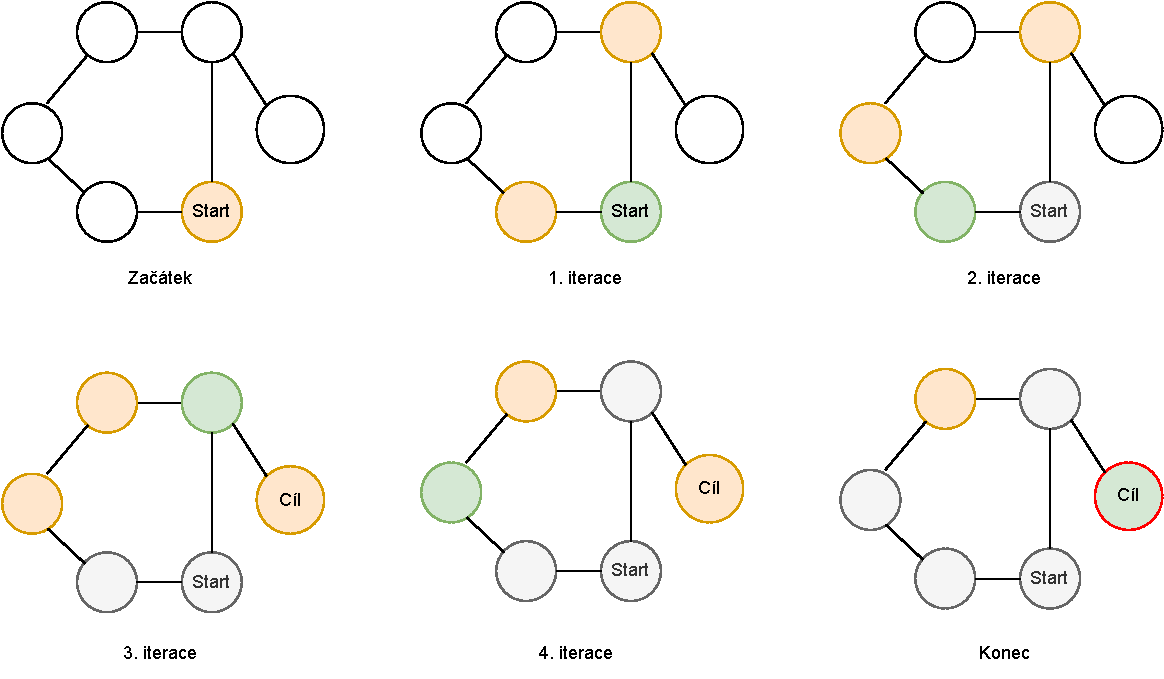
\includegraphics[width=\textwidth]{assets/img/bfs.pdf}
    \caption{Běh algoritmu BFS}
    \label{fig:bfs}
\end{figure}


Pomocí tohoto algoritmu je tedy zjištěna nejkratší cesta do dané sítě. Tato cesta je nalezena v nejhorším případě v komplexitě $O(|V| + |E|)$, kde $|V|$ je počet uzlů, neboli kontejnerizovaných zařízení, a $|E|$ je počet hran mezi uzly, neboli spojení mezi zařízeními. \cite{pruvodce_alogritmu} Zároveň metoda pro každé zařízení může být volána maximálně $|V| - 1$ krát. Tyto vlastnosti jsou naprosto dostačující pro aktuální použití.

Metoda tedy navrací seznam zařízení, bez počátečního zařízení, který reprezentuje cestu od počátečního zařízení do cílového zařízení, neboli do dané sítě. Podstatnou informací je první položka v seznamu, tedy to sousední zařízení, kterému musí být zpráva odeslaná z daného zařízení, aby dosáhla cílového. To je nastaveno jako směr, kterým mají být všechny zprávy do dané sítě odesílány. Tímto způsobem implementace je testovací knihovna schopna nastavit všechny požadované topologie. Zároveň vždy odesílá zprávy nejkratší možnou cestou.

\subsection{Správa kontejnerů}\label{sec:cont_managment}

Stejně jako síť, i kontejnery mají svého správce, realizovaného třídou \inlinecode{ContainerManager}. Každý kontejner je podobně jako v případě sítí registrován s pomocí metody \inlinecode{AddContainer(string, ContainerConf)}, kde metoda obdrží v argumentech název a nastavení zařízení, získaného z konfiguračního souboru. To je uloženo do fronty pro následné zpracování.

Po přidání všech zařízení je možné zavolat metodu \inlinecode{Build}. Ta očekává jako argument instanci třídy \inlinecode{NetworkManager}, která již má vypočítané nastavení sítě daných zařízení. Nastavení pro jednotlivé zařízení jsou získávána za pomoci metody \inlinecode{NetworkManager.GetContainerConf(string)}, kde argumentem je název zařízení. 

Metoda \inlinecode{Build} následně zpracovává všechna zařízení ve frontě. Pokud obraz na zařízení je definován za pomoci Dockerfile, tak poté před vytvořením zařízení metoda \inlinecode{BuildImage} sestaví daný obraz. Metoda nejdříve zkontroluje, zdali daný obraz z Dockerfile již nevytvořila. Tuto kontrolu provádí tím, že při vytvoření si uloží hash zdrojového souboru do slovníku \inlinecode{imageTags}, kde hash souboru je klíčem a následně název vytvořeného obrazu je hodnotou ve slovníku. Po zajištění existence obrazu tedy metoda \inlinecode{BuildImage} vrátí název odpovídajícího obrazu. 

Vytvoření samotného kontejneru je následně provedeno metodou \inlinecode{CreateContainer}. Ta dostane jako argument název zařízení, název obrazu, instanci nastavení zařízení a instanci nastavení sítě zařízení. 

Každá kontejner je definovaný za pomoci rozraní \inlinecode{IVMContainer}, definovaného v sekci \ref{sec:cont_design}. Pomocí jeho metod je každý kontejner nastavován a realizace těchto nastavení je poté na dané implementaci rozhraní. V aktuální implementaci existují tyto dvě implementace kontejnerů: 

\begin{itemize}
    \item \inlinecode{DefaultContainer} - základní kontejner vycházející z operačního systému Ubuntu. Reprezentován je hodnotou z výčtového typu \inlinecode{ContainerType.DEFAULT} 
    \item \inlinecode{NetworkLogger} - kontejner, který zajišťuje odposlouchávání sítě. Reprezentován je hodnotou z výčtového typu \inlinecode{ContainerType.NETWORK\_LOGGER}
\end{itemize}

Oba dva typy kontejnerů jsou rozlišeny za pomoci výčtového typu \inlinecode{ContainerType}. Každá jeho hodnota by měla být napsána velkými písmeny. V konfiguračním souboru se následně preferuje verze s malými písmeny, i když jakákoliv kombinace velkých a malých písmen bude akceptována. 

Následně rozšiřující statická metoda výčtového typu \inlinecode{GetInstance} dokáže vytvořit instanci daného typu kontejneru. Metoda zároveň obdrží argumenty pro konstruktor daného kontejneru. Hlavními argumenty jsou název kontejneru a název obrazu kontejneru. Kontejner typu \inlinecode{NetworkLogger} může ještě obdržet instanci třídy \inlinecode{ServiceConfiguration}, díky které obdrží nastavení testovací služby, ke které se následně připojí. 

Metoda \inlinecode{CreateContainer} následně vrátí instanci kontejneru, která je následně uložena do slovníku \inlinecode{containers}, kde klíčem je název zařízení. 

\subsection{Správce celého virtualizovaného prostředí}

Předchozí zmíněné správce je potřeba orchestrovat společně. K tomuto slouží třída \inlinecode{VirtualEnvironmentManager}. Třída obdrží instanci \inlinecode{EnvironmentConfiguration}, která reprezentuje nastavení virtualizovaného prostředí definovaného v sekci \ref{sec:env_conf}. Následně také obdrží instanci třídy \inlinecode{ServiceConfiguration}, ve které je obsaženo nastavení testovací služby.

Třída v sobě obsahuje instance obou dvou správců \inlinecode{NetworkManager} a \inlinecode{ContainerManager}. V konstruktoru je zavolána metoda \inlinecode{SetupEnvironment}, která zaregistruje všechny zařízení a připojení mezi nimi. Zároveň, pokud dle nastavení je potřeba zachytávat na daném spojení komunikaci, tak také přidá adekvátně dané odposlouchávače komunikace. 

Zavoláním metody \inlinecode{Build} je následně vytvořeno celé prostředí. Nejdříve je vytvořena požadovaná síť a následně jsou vytvořeny všechny kontejnery. Na konci metoda spustí všechny kontejnery.

Za pomoci metody \inlinecode{Stop} je poté následně možné zastavit všechny kontejnery. Nakonec, metodou \inlinecode{Dispose} jsou následně odstraněny všechny vytvořené prostředky prostřednictvím daných správců. 

\subsection{Ošetření chyb}

Implementace virtualizovaného prostředí ošetřuje všechny chyby tím, že v případě jejich vzniku vyhodí odpovídající výjimku. Je tedy potřeba následně tyto chyby v případě jejich vzniku zachytávat a adekvátně vyhodnotit.

Ovšem pokud je program násilně ukončen, tak může dojít k nesmazaní daných vytvořených prostředků v Docker prostředí. To může způsobit jejich akumulaci a v případě sítě dokonce selhání vytvoření sítě. Testovací knihovna proto definuje ve statické třídě \inlinecode{TestLibConstants} proměnnou \inlinecode{ResourcePrefix}, který je přidán ke všem vytvořeným prostředkům.

Díky tomu může knihovna identifikovat jím vytvořené prostředky. Každý správce má tedy implementovanou metodu pro odstranění zbylých prostředků. Ty jsou volány prostřednictvím metody \inlinecode{RemoveHangingResources} v konstruktoru správce virtualizovaného prostředí před započetím všech akcí k vytvoření nového prostředí.

\subsection{Definice kontejnerů}

Jak jsem zmínil v sekci \ref{sec:cont_managment}, aktuálně testovací knihovna definuje dvě zařízení. Zařízení typu \inlinecode{default} je výchozím zařízením pro všechny aktuální kontejnery. Zařízení vychází z operačního systému Ubuntu 22.04. 

Ke správné orchestraci zařízení potřebuje kontejnerizované zařízení obsahovat potřebné nástroje k nastavení sítě. Všechny tyto nástroje jsou definované v novém obraze nazvaném \inlinecode{testlib-ubuntu-base}. Obraz obsahuje tyto balíčky:

\begin{itemize}
    \item \inlinecode{net-tools}
    \item \inlinecode{iproute2}
\end{itemize}

Všechny kontejnery, které budou vycházet z tohoto obrazu, bude možné použít v testovací knihovně. Tento obraz byl zveřejněn ve veřejném repositáři na Docker Hub\cite{docker_hub}, kde je dostupný pod názvem \inlinecode{wheeeper/testlib-ubuntu-base}.

Označení verze obrazu bude kopírovat označení podkladového obrazu operačního systému Ubuntu. Tedy verze bude stejná jako verze operačního systému Ubuntu. 

Následná definice kontejnerů v konfiguračním souboru virtualizovaného prostředí bude probíhat dle definice v \ref{sec:env_conf}. Je ovšem potřeba zajistit, že všechny cesty v konfiguraci budou pro program dostupné, či validní. V případě relativních cest uvnitř konfiguračního souboru bude knihovna pokládat umístění konfiguračního souboru jako výchozí bod pro dané relativní cesty.

\subsection{Odposlouchávání komunikace}

K odposlouchávání komunikace byl vytvořen nový program pod názvem \inlinecode{NetworkLogger}. Program využívá knihovnu SharpPcap\cite{sharppcap} pro zachytávání komunikace na daném virtuálním rozhraní. 

Program přijímá variabilní počet argumentů v závislosti na módu fungování. Program podporuje dva módy fungování

\begin{enumerate}
    \item Mód bez připojení k testovací službě
    \item Mód s připojením k testovací službě
\end{enumerate}

K aktivaci prvního módu je potřeba předat programu přepínač \inlinecode{--no-service}, který mód aktivuje. Následně program očekává seznam názvů rozhraní, oddělených mezerou, ze kterých má zachytávat komunikaci. Při spuštění program zachytává všechnu komunikaci na daných rozhraní a následně vypisuje jednotlivé zachycené zprávy na standardní výstup.

V druhém implicitně definovaném módu testovací knihovna očekává tyto poziční argumenty:

\begin{enumerate}
    \item Složku, kde bude ukládat zachycené zprávy do souboru.
    \item Adresu, na které běží testovací služba.
    \item Port, na kterém běží testovací služba.
    \item Variabilní počet jmen rozhraní, které má zaznamenávat, oddělený mezerou.
\end{enumerate}

Ilustraci úspěšného běhu s jedním testem můžeme vidět na diagramu aktivit, který je na obrázku \ref{fig:logger_activity}. Jak je vidět, po obdržení argumentů se program připojí k testovací službě a projde stejnou inicializační fází, jako všichni ostatní účastníci testu. Následně po obdržení zprávy o započnutí testu začne zaznamenávat síť. Program využívá separátních vláken pro záznam komunikace a pro zpracovaní jednotlivých paketů. Díky tomuto přístupu není omezen výkon zaznamenávání například zápisem do souboru. Všechny přijaté pakety mohou být tedy ihned zapsány. 

Zaznamenávání sítě je ukončeno při obdržení zprávy o ukončení testu. Jednotlivé testy jsou tedy zaznamenávány separátně a pro každý test je vytvořen separátní záznam, rozlišen identifikátorem testu. Zároveň je ovšem kontrolována kolize záznamů a jméno výstupního souboru je v případě kolize upraveno. 

\begin{figure}[htbp]
    \centering 
    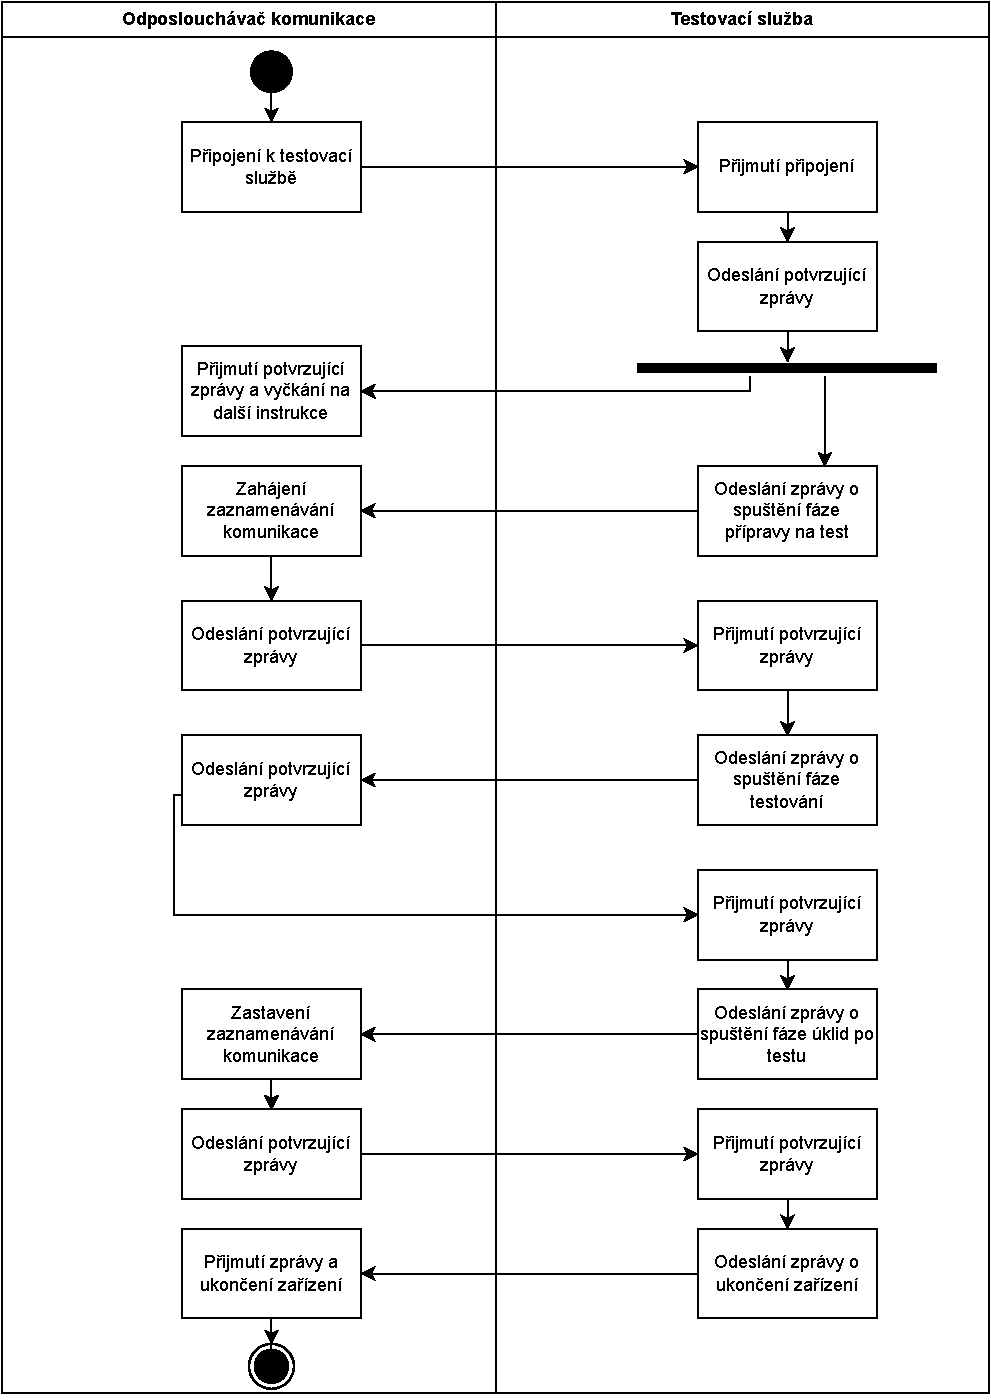
\includegraphics[width=0.95\textwidth]{assets/img/activity_networklogger.pdf}
    \caption{Aktivity diagram odposlouchávače komunikace}
    \label{fig:logger_activity}
\end{figure}

Program má definovaný Dockerfile, vycházející z definovaného obrazu \inlinecode{testlib-ubuntu-base}, na základě něhož může být program spuštěn ve virtualizovaném prostředí prostřednictvím softwaru Docker. Ten je oproti původnímu prostředí rozšířen o dvě komponenty:

\begin{itemize}
    \item \inlinecode{dotnet-runtime-6.0} - vše potřebné ke spuštění .NET 6 programu v Ubuntu
    \item \inlinecode{libpcap-dev} - knihovna k zaznamenávání packetů 
\end{itemize}

Obraz také využívá obraz \inlinecode{mcr.microsoft.com/dotnet/sdk:6.0}, s pomocí než je celý program zkompilován. V základním nastavení je program spuštěn v módu bez připojení k testovací službě. To lze při vytváření kontejneru změnit a tedy program správně nastavit. Daný vytvořený obraz byl zveřejněn ve veřejném repositáři na Docker Hub\cite{docker_hub} a je dostupný pod názvem \inlinecode{wheeeper/networklogger}.

\section{Integrace virtualizovaného prostředí do testovací knihovny}

Pro integraci virtualizovaného prostředí je potřeba integrovat virtualizované prostředí do služeb testovací knihovny. Původní třída \inlinecode{ServiceRunner} byla přejmenovaná na \inlinecode{ServicesRunner}, aby název lépe reflektoval její zónu odpovědnosti. Ta v sobě obsahuje instance tříd \inlinecode{TestService} a \inlinecode{VirtualEnvironmentManager}.

Do statické třídy \inlinecode{API} byla přidána statická metoda \inlinecode{BuildEnvironment}. Tato metoda obdrží v argumentu cestu ke konfiguračnímu souboru daného virtualizovaného prostředí. Metoda načte danou konfiguraci a následně zavolá metodu \inlinecode{ServiceRunner.StartServices(EnvironmentConfiguration)}. Za pomoci ní je vytvořeno dané virtualizované prostředí. Nejdříve je ovšem zkontrolováno, zdali dané prostředí již není vytvořeno. Pokud ano, metoda ponechává dříve vytvořené prostředí. V opačném případě metoda ukončí testovací službu a zničí předchozí virtualizované prostředí (pokud nějaké existuje). Následně na to vytvoří nové virtualizované prostředí. Po úspěšném vytvoření prostředí je následně spuštěna testovací služba.

Použití této funkce je zamýšleno v rámci jednotlivých tříd testů. Testovací knihovna používá knihovnu MSTest pro propojení se serverem Azure DevOps, který může automaticky spouštět jednotlivé testy. Všechny testy musí být shlukovány do jednotlivých testovacích tříd. Testovací knihovna MSTest definuje atribut \inlinecode{ClassInitialize}. Metoda s tímto atributem bude spouštěna právě jednou před započetím testů v dané třídě. Je tedy logické shlukovat jednotlivé testy dle konfigurace virtualizovaného prostředí. Tímto použitím se minimalizuje riziko zbytečného přestavování virtualizovaného prostředí. 

Třída \inlinecode{API} také nově definuje metodu \inlinecode{SetServiceConfig}, díky které může být změněno základní nastavení testovací služby, jenž je popsáno v sekci \ref{sec:test_service_changes}.


